% title: 곡선과 접선
% description: 곡선 y = f(x) 위의 점 (a, f(a))에서 그은 접선 y = f'(a)(x - a) + f(a). 접점 표시와 점선 보조선
% packages: pgfplots
% libraries:
% f를 바꾸면 도함수 df도 같이 바꾼다. a는 접점의 x좌표.
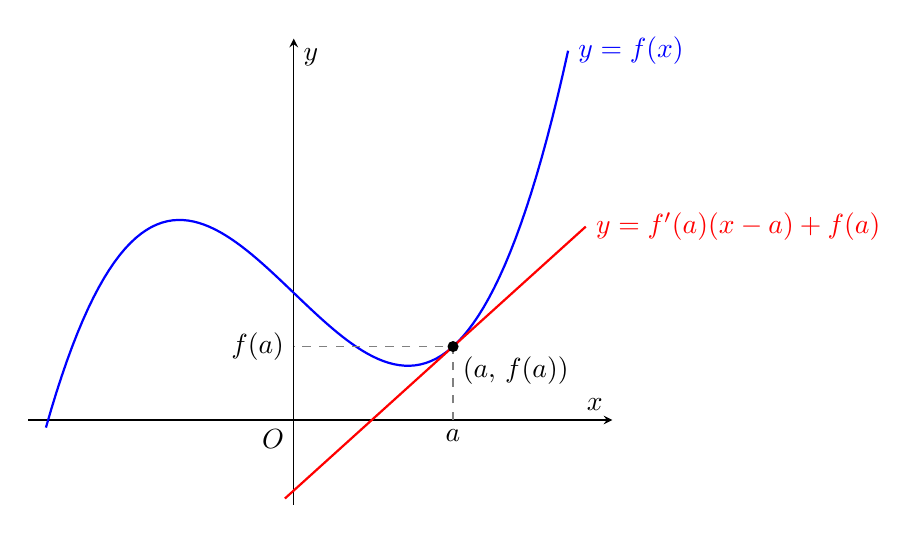
\begin{tikzpicture}[declare function={
    f(\x)  = 0.2*\x^3 - \x + 1.5;
    df(\x) = 0.6*\x^2 - 1;
  }]
  \def\a{1.8}
  \begin{axis}[
      width=9cm, height=7.5cm,
      axis lines=middle, xmin=-3, xmax=3.6, ymin=-1, ymax=4.5,
      xlabel={$x$}, ylabel={$y$}, xtick=\empty, ytick=\empty,
      samples=100, clip=false]
    \addplot[thick, blue, domain=-2.8:3.1] {f(x)} node[right] {$y=f(x)$};
    \addplot[thick, red, domain=\a-1.9:\a+1.5] {df(\a)*(x-\a) + f(\a)}
      node[right] {$y=f'(a)(x-a)+f(a)$};
    \draw[dashed, gray] (\a,0) -- (\a,{f(\a)}) -- (0,{f(\a)});
    \fill (\a,{f(\a)}) circle[radius=2pt] node[below right] {$(a,\,f(a))$};
    \node[below] at (\a,0) {$a$};
    \node[left] at (0,{f(\a)}) {$f(a)$};
    \node[below left] at (0,0) {$O$};
  \end{axis}
\end{tikzpicture}
